% File: design.tex
% Date: 8.27.2014
% Author: Jared Bold

% Section Name
\chapter{Design}

% Common Design Components
\section{Common Design Components}

% Image format
\subsection{Tagged Image File Format}
All images used throughout this research are Tagged Image File Format (TIFF) images. TIFF images consist of an image header that describes the byte order, TIFF version number, and offset to the image file directory\cite{Wiggins2001}.  The image file directory stores the offsets to the directory entries and varies in size based on the number of images contained within the TIFF image.  The directory entry is then broken down into several sections including a Tag section which consists of a number of tags which give information about the image including the bits per pixel, compression scheme, image length and height, and many more.  The directory entry is lastly completed with the offset to the image data. Figure \ref{fig:tiffFormat} shows a more indepth representation of the TIFF structure for multiple image TIFFs.

\begin{figure}
  \centering
  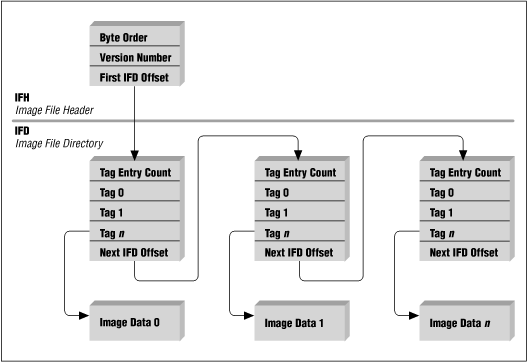
\includegraphics[width=10cm]{./img/tiffFormat.png}
  \caption{TIFF File Structure\cite{Murray1996}}
  \label{fig:tiffFormat}
\end{figure}

For the purposes of this research, only uncompressed TIFF images are used in order to eliminate the need for resource intensive decompression and compression of input and output images.  To support the reading and writing of these image files, the LibTiff libary is cross-compiled for use on the ZC702's PetaLinux OS. 

\subsection{User Interface}
A common user interface (UI) was developed for each algorithm in order to maintain continuity as well as ease development.  The UI shown in figure \ref{fig:ui} is used to fully test, validate, and exercise the C and hardware implementations of the 3x3 Gaussian blur filter.  The UIs for the 9x9 Laplacian of Gaussian filter and bilinear interpolation algorithms are identical with the exception of the title shown above the selection options.  From the UI, the user is prompted with an option selection; which based on the input performs different operations.  Selection option 1 runs the C version of the algorithm only, displays the runtime of a single run of the algorithm, and also outputs the resulting output image to a TIFF image file.  Selecting option 2 runs the hardware version of the algorithm, displays the runtime of a single run of the algorithm in hardware, and also outputs the resulting output image to a TIFF image file.  Selecting option 3 runs both the C and hardware versions of the algorithm and compares the outputs pixel by pixel.  This is used to verify that the hardware implementation yields an identical output as the software algorithm.  Depending on the algorithm, border pixels may be ignored due to the use of unitialized values resulting in inconsistancies not only between the hardware and software implementations, but also between runs in these regions.  Selecting option 4 performs the C and hardware implementations 500 times and displays the average runtimes for each.

\begin{figure}[t]
  \centering
  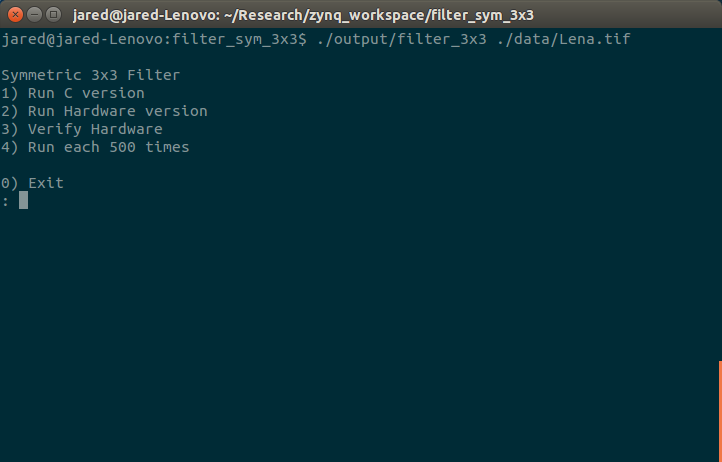
\includegraphics[width=0.9\textwidth]{./img/research_ui.png}
  \caption{User Interface}
  \label{fig:ui}
\end{figure}

\section{Processor Based Design}

\subsection{Image Filter}
For this experiment, two filter kernels are used.  The first is a 3x3 Gaussian blur filter and the second is a 9x9 Laplacian of Gaussian (LoG) filter.  The framework in the processor based design is the same for both of these kernels as shwon in Figure \ref{fig:filter_soft_framework}.  The processing occurs in the following steps:
\begin{enumerate}
  \item Read in the TIFF input image from the file system
  \item Allocate the output image in memory
  \item Peform the filtering by applying the filter kernel pixel by pixel, iterating over the entire image
  \item Convert the output image to the TIFF specification
  \item Write the TIFF output image to the file system
\end{enumerate}

\begin{figure}[h]
  \centering
  %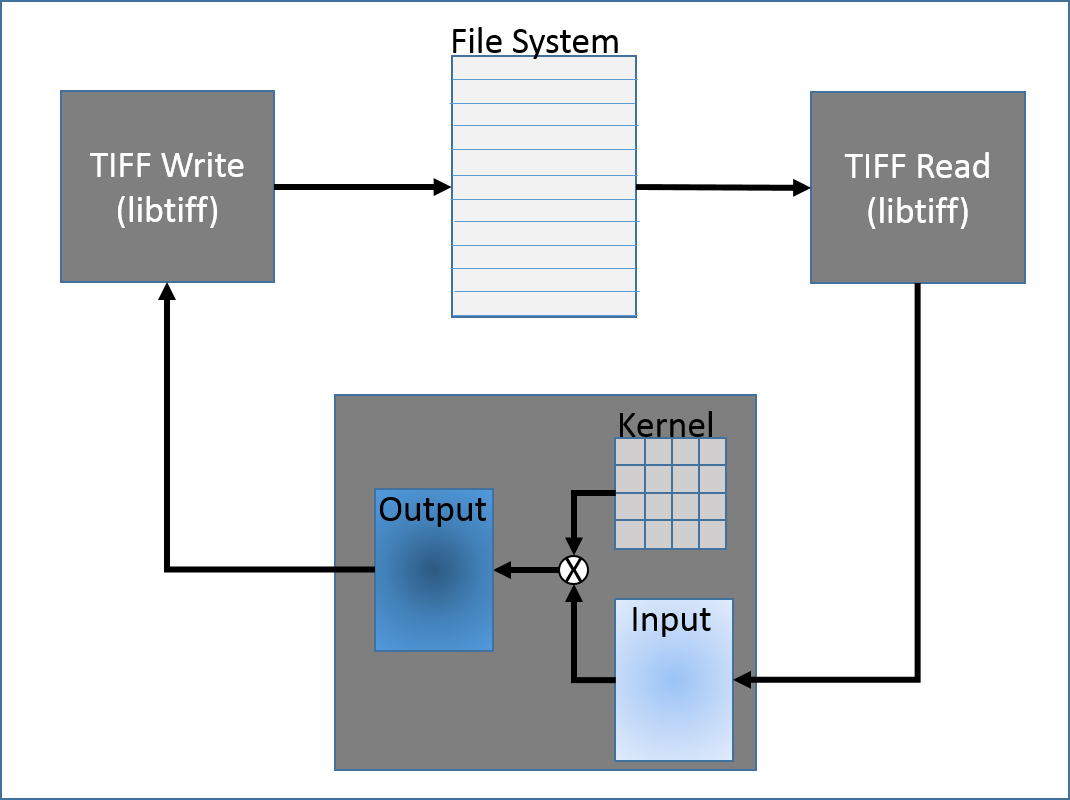
\includegraphics[width=0.9\textwidth]{./img/filter_software_framework.png}
  \caption{Processor based filter framework}
  \label{fig:filter_soft_framework}
\end{figure}

Since the Linux operating system is used, the Zynq device provides a static file system that is used to store the input and output images.  This file system eliminates the need to transmit the processed image back to a host machine for storage.

\subsubsection{3x3 Gaussian Blur Filter}
\begin{figure}[h]
  \centering
  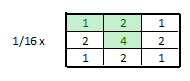
\includegraphics{./img/filter_3x3_values.PNG}
  \caption{3x3 Gaussian blur filter kernel}
  \label{fig:3x3_filter}
\end{figure}

The 3x3 Gaussian blur filter used in this experiment is shown in Figure \ref{fig:3x3_filter}. The filter acts as smoothing filter, removing some of the higher spactial frequencies present in the image and has a blurring effect.  The scale factor in front of the filter normalizes the filter so that there is no overall gain in the output image.

\subsubsection{9x9 Laplacian of Gaussian Filter}
\begin{figure}[h]
  \centering
  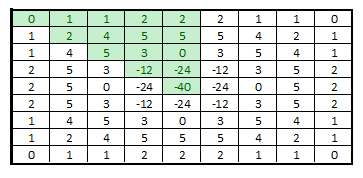
\includegraphics{./img/filter_9x9_values.PNG}
  \caption{9x9 LoG filter kernel}
  \label{fig:9x9_filter}
\end{figure}

The 9x9 LoG filter used in this experiment is shown in \ref{fig:9x9_filter}.  The filter is the equivalent of applying a Gaussian smoothing filter followed by a Laplacian high pass filter to an input image.  The reason that this is typically employed is to reduce the noise in an image using the smoothing filter and then to extract the edges within the image using the high pass filter.  Since the output image is high pass filtered, the mean value (DC component) is removed and the resulting output can be either a postive or negative number that would be unable to be displayed in a standard image format.  To resolve this issue, each output pixel is offset by 128 in order to remove any negative numbers.  Unlike the Gaussian blur filter, there is no need for a scale factor when applying the LoG filter because all of the coefficients sum to 0.

\subsection{Bilinear Interpolation}

\section{Programmable Logic Based Design}

\subsection{Image Filter}
\subsubsection{3x3 Gaussian Blur Filter}
\subsubsection{9x9 Laplacian of Gaussian Filter}

\section{Homogeneous Design}
\subsection{Bilinear Interpolation}

